\documentclass[12pt, french]{article}

\usepackage{fancyhdr, fancybox, lastpage}
\usepackage[most]{tcolorbox}
\usepackage[a4paper, margin={0.3in, .75in}]{geometry}
\usepackage[siunitx, RPvoltages]{circuitikz}
\usepackage{wrapfig}
\pagestyle{fancy}
\renewcommand\headrulewidth{1pt}
\renewcommand\footrulewidth{1pt}
\fancyhf{}
\rhead{ \em{Zakaria Haouzan}}
\lhead[C]{\em{1ére année baccalauréat Sciences Mathématiques}}
\chead[C]{}
\rfoot[C]{}
\lfoot[R]{}
\cfoot[]{\em{Page \thepage / \pageref{LastPage}}}


\newtcolorbox{Box2}[2][]{
                lower separated=false,
                colback=white,
colframe=white!20!black,fonttitle=\bfseries,
colbacktitle=white!30!gray,
coltitle=black,
enhanced,
attach boxed title to top left={yshift=-0.1in,xshift=0.15in},
title=#2,#1}


\begin{document}
\begin{center}
   \shadowbox {\bf{Forces électromagnétiques }}
\end{center}


%%_________________________Exercice ! :"_________________________Exercice
   \begin{Box2}{Exercice 1 : champ
      magnétique $\vec{B}$/Force de Laplace$\vec{F}$  }
Représenter, dans chacun des cas suivants, le sens et la direction du courent électrique, du champ
magnétique ou de la force de Laplace :
  \begin{center}
     \vspace{-0.5cm}
    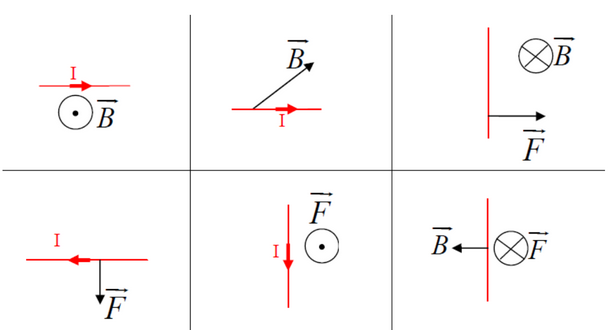
\includegraphics[width=0.5\textwidth]{./img/Ex_00.png}
  \end{center}


   \end{Box2}


%%_________________________Exercice !2 :"_________________________Exercice
\begin{Box2}{Exercice 2 :Forces électromagnétiques }
On considère le montage expérimental représenté dans ci-dessous dans lequel AB est une tige homogène de longueur
$L=20cm$ et de masse $m=12mg$ , capable de tourner sans frottement autour d'un axe fixe $( \Delta)$ horizontal passant le point A.

   La tige passe dans l'entrefer d'un aimant en U créant un champ magnétique uniforme qui s'étend sur une largeur $d = \frac{L}{4}$

comme l'indique la figure ci-dessous .
L'axe de symétrie de la région ou règne le champ magnétique se trouve à une distance h du point A (voir figure).
  \begin{center}
     \vspace{-0.5cm}
    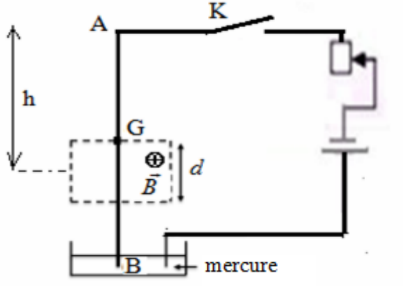
\includegraphics[width=0.3\textwidth]{./img/Screenshot from 2022-05-11 19-05-37.png}
  \end{center}


Lorsqu'on ferme le circuit, un courant électrique continu d'intensité I=10A passe dans la tige du point B au point A et elle s'incline d'un angle $\alpha = 40^{\circ}$
puis elle se stabilise.

1. Quelle est la cause de l'inclinaison de la tige ? Justifier votre réponse. 

2. Soit le point C : point d'application de la force qui a provoquer l'inclinaison de la tige . Indiquer sur la figure la position
de ce point en justifiant votre réponse, puis représenter cette force dans la position verticale de la tige.

3.Faire le bilan des forces qui s'appliquent sur la tige à l'équilibre puis représenter ces forces sur une figure dans la
position d'équilibre.

4. Donner l'expression de la force qui a provoqué l'inclinaison de la tige et préciser son sens et sa direction.

5. Donner l'expression l'intensité de la force qui a provoqué l'inclinaison de la tige en fonction de I, B et L.

6. Le point G étant le centre d'inertie de la tige .Exprimer la distance h en fonction de L .

   7. En appliquant le théorème des moments, montrer que l'intensité de la force qui a provoqué l'inclinaison de la tige est  $F = \frac{4}{5}.m.g.sin\alpha$ 

   8. En déduire l'expression de l'intensité du champ magnétique en fonction de m, g , L et $\alpha$ . puis calculer sa valeur.
\end{Box2}
\begin{center}
   \Large{ \em{Exercices Supplémentaires}}
\end{center}


%%_________________________Exercice 4 : _________________________Exercice
\begin{Box2}{Exercice 3 : Rails Conducteurs}
\begin{wrapfigure}{r}{0.3\textwidth}
  \begin{center}
     \vspace{-0.5cm}
    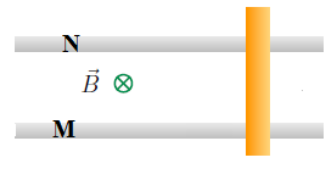
\includegraphics[width=0.3\textwidth]{./img/Rails_00.png}
  \end{center}
\end{wrapfigure}
Une tige en cuivre de $20 cm$ de longueur et $250 g$ de masse repose sur deux rails conducteurs distants de $15cm$ et disposés dans un plan horizontal. Le dispositif est placé dans un champ magnétique uniforme
d'intensité $B = 0,3 T$.

1. Comment peut-on créer un champ magnétique uniforme? Citer deux exemples.

2. On branche un générateur de courant continu à ce dispositif: le pôle positif en
N, le pôle négatif en M. Représenter sur une figure la force magnétique exercée sur la tige et calculer sa
valeur si l’intensité du courant vaut 10 A.

3. Quel doit être l’angle d’inclinaison du rail par rapport au plan horizontal pour que la tige soit en équilibre ?

\end{Box2}
%\vspace{2cm}
%%_________________________Exercice 5 : _________________________Exercice
\begin{Box2}{Exercice 4 : haut-parleur électromagnétique }

Un haut-parleur électromagnétique est constitué d’un aimant permanent de forme particulière, et d’une
bobine parcourue par un courant et pouvant coulisser sur l’un des pôles de l’aimant. La bobine est solidaire
d’une membrane M. (schéma ci-contre)
  \begin{center}
     \vspace{-0.5cm}
    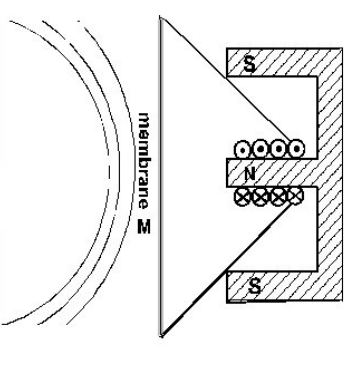
\includegraphics[width=0.4\textwidth]{./img/Haut_parleurs.png}
  \end{center}
   1. On suppose que le courant dans la bobine est continu.

   1.1. Représenter par un vecteur le champ magnétique existant au
niveau des conducteurs.

   1.2. En déduire la direction et le sens des forces électromagnétiques exercées sur chaque spire de la bobine
   
   1.3. Quel est l’effet de ces forces sur la membrane M ?

   2. En réalité, le courant appliqué à la bobine est variable.

   2.1.Quel est l’effet de ce courant sur la membrane ?

   2.2. Pourquoi obtient-on un son ?

\end{Box2}
%%_________________________Exercice 6 : _________________________Exercice
\end{document}
